\clearpage\section {Класове I: Прости класове, методи и оператори}

\begin{enumerate}


\item Задача 2.39.\cite{sbornik2} Да се дефинира клас \texttt{Time}, който определя момент от денонощието по зададени час и минути. Класът да съдържа подходящи методи за:

\begin{itemize}

 \item достъп и промяна на часа и минутите с проверки за коректност;
 \item добавящ към времето цяло число минути;
 \item достъп до боря минути, изминали от началото на денонощието;
 \item оператор за сравнение (казваме, че $t_1 < t_2$, ако $t_2$ е по-късно в денонощието от $t_1$).

\end{itemize}


Да се предефинират операторите +, - и *, така че да могат да се събират и изваждат две времена, както и да се умножават време с цяло число и цяло число с време. Да се включи дефинираният клас в програма и направят обръщения към член-функциите му и предефинираните оператори.

\item Да се дефинира структура \code{Point}, описваща точка в евклидовата равнина и клас  \code{Line}, описващ права в евклидовата равнина, зададена чрез две нейни точки.

Класът \code{Line} да съдържа методи, чрез които може да се извършват следните операции:

\begin{itemize}
	\item Проверка дали две прави са успоредни;
	\item Проверка дали дадена точка лежи на дадена права;
	\item Намиране на пресечната точка на две прави. Приемаме, че правите не са успоредни. Стойността на резултата може да е произволна в противен случай.
	\item Създаване на права, която е ъглополовяща на по-големия ъгъл, образуван от две прави. Стойността на резултата може да е произволна в противен случай.
\end{itemize}

Където е подходящо да се дефинират оператори вместо методи.


\item Задача 2.44. \cite{sbornik2} (асоциативен масив) Да се дефинира клас \texttt{Dictionary}, който създава тълковен речник. Тълковният речник се състои от не повече от 500 двойки дума–тълкувание, като думата е символен низ с не повече от 100 символа, а тълкованието е символен низ с не повече от 500 символа.

\begin{itemize}
	\item Да се дефинира подходяща структура, описваща една двойка дума-тълкувание;
	\item Да се дефинират подходящи член-данни на клас \texttt{Dictionary};
\end{itemize}

Клас \texttt{Dictionary} да съдържа методи, с които може да се извършват следните операции над речника:

\begin{itemize}

\item Инициализация на празен речник;
\item извеждане на всички думи в речника и техните тълкувания;
\item включване на нова двойка дума–тълкуване в речника;
\item изключване на двойка дума–тълкуване от речника (по дадена дума);
\item търсене на значението на дадена дума в речник.
\item извеждане на всички думи в речника и техните тълкувания по азбучен ред на думите;
\end{itemize}

Да се дефинира оператор +, обединяващ два речника, такъв че:

\begin{itemize}
 \item Ако някои думи имат значение и в двата речника, значенията да се конкатенират в резултатния сумарен речник;
 \item Ако общият брой на думите в двата речника надхвърля 500, да се използват само първите 500 думи (при произволна наредба).
\end{itemize}


\end{enumerate}


\pagebreak

\clearpage\section {Жизнен цикъл на обектите}

\subsection {Конструктори}

\begin{enumerate}

\item Да се дефинира клас Word, описващ дума, съставена от не повече от 20 символа от тип char. Класът да съдържа следните операции:

\begin{itemize}
\item оператор \code{[]} за намиране на \code{i}-тия пореден символ в думата
\item оператори \code{+} и \code{+=} за добавяне на един символ в края на думата. Ако думата вече има 20 символа, операторите да нямат ефект
\item оператори \code{<} и \code{==} за сравнение на думи спрямо лексикографската наредба
\item подходящи конструктори

\end{itemize}

Да се реализира и изпълни подходящ тест за класа и неговите методи.


\item Да се реализира клас \code{NumbersSummator},  който поддържа сума на цели числа. При създаване на обект от класа,  съответната му сума да се инициализира с число, което се подава като аргумент на конструктора. За класа да се реализират следните методи:

\begin{itemize}
\item sum, който връща текущата стойност на сумата
\item add, увеличаващ сумата с дадено число
\item sub, намаляващ сумата с дадено число
\item num, връща колко пъти сумата е била променяна
\item average, връщащ средното аритметично на всички числа, с които сумата е била променяна.

\end{itemize}


\textit{Забележка:}Функционалност извън тези 4 метода, като например съхраняване на отделните числа от поредицата, не е необходима.
Пример:
\begin{lstlisting}

	NumbersSummator seq1 (10);
	seq1.add (10);
	seq1.add (5);
	seq1.sub (15);
	cout << seq1.sum() ; //->10 (10+10+5-15)
	cout << seq1.average(); //->0 (10+5-15)/3

\end{lstlisting}



\item \label{zad:browser} Да се дефинира клас \code{BrowserHistory}, който съдържа информация за историята на посещението до най-много \code{N} Web сайта. \code{N} е параметър на конструктора на класа. За целта да се реализира структура \code{HistoryEntry}, описваща едно посещение на сайт чрез:

\begin{enumerate}[label=\alph*)]
	\item Месец от годината, през който е посетен сайтът;
	\item Неговото URL.
\end{enumerate}

Класът code{BrowserHistory} да поддържа следните операции:
\begin{itemize}
\item Метод за добавяне на нов сайт към историята. Информацията за всеки сайт се въвежда от клавиатурата
\item Оператор += с параметър \code{HistoryEntry}, добавящ сайт към историята
\item Метод за отпечатване на информацията за всички сайтове в историята
\item Метод, който по даден месец от годината намира броя на сайтовете, посетени през този месец
\item Намиране на този месец от годината, в който има най-много посетени сайтове
\item Премахване на най-скоро добавеният сайт в историята
\item Оператор +, който обединява двете истории
\end{itemize}

Да се реализира и изпълни подходящ тест за класа и неговите методи.

\end{enumerate}

\pagebreak

\subsection{Копиране}

\begin{enumerate}[resume]

  \item За клас \code{BrowserHistory} от задача \ref{zad:browser} да се реализират конструктор за копиране, оператор за присвояване, оператори за събиране \code{+} и \code{+=}, обединяващи две истории и деструктор.\\

  Да се реализира подходящ тест на класа.

  \item Задача 2.2.44. (асоциативен масив) \cite{sbornik2}\label{zad:dict1} Да се дефинира клас \texttt{Dictionary}, който създава тълковен речник. Тълковният речник се състои от не повече от 500 двойки дума–тълкувание, като думата е символен низ с не повече от 100 символа, а тълкованието е символен низ с не повече от 500 символа.

  \begin{itemize}
  	\item Да се дефинира подходяща структура, описваща една двойка дума-тълкувание;
  	\item Да се дефинират подходящи член-данни на клас \texttt{Dictionary};
  \end{itemize}

  Клас \texttt{Dictionary} да съдържа методи, с които може да се извършват следните операции над речника:

  \begin{itemize}

  \item Инициализация на празен речник;
  \item извеждане на всички думи в речника и техните тълкувания;
  \item включване на нова двойка дума–тълкуване в речника;
  \item изключване на двойка дума–тълкуване от речника (по дадена дума);
  \item търсене на значението на дадена дума в речник.
  \item извеждане на всички думи в речника и техните тълкувания по азбучен ред на думите;
  \end{itemize}

  Да се дефинира оператор +, обединяващ два речника, такъв че:

  \begin{itemize}
   \item Ако някои думи имат значение и в двата речника, значенията да се конкатенират в резултатния сумарен речник;
   \item Ако общият брой на думите в двата речника надхвърля 500, да се използват само първите 500 думи (при произволна наредба).
  \end{itemize}


  \item Клас \code{Dictionary} от задача \ref{zad:dict1} да се реализира така, че максималният брой \code{N} на двойки ключ-стойност, които могат да бъдат добавени към речника, да се задава като параметър на конструктора на класа. За класа да се реализират конструктор за копиране, оператор за присвояване и деструктор.\\

 Да се реализират оператори за събиране \code{+} и \code{+=}, обединяващи два речника. Ако в речниците \code{a} и \code{b} има еднакви думи с различни значения, то за тези думи в речника \code{a+b} да се използва значението им от речника \code{a}. \\

 Да се реализира подходящ тест на класа.

\end{enumerate}
\begin{mdframed}[hidealllines=true,backgroundcolor=gray!20]
Някои от следващите задачи са върху примерния шаблон \code{Vector}, разработен на лекции. Шаблонът реализира прост контейнер чрез масив в динамичната памет:
\begin{verbatim}
template <typename T>
class Vector
{
public:
    Vector();
    Vector(const Vector<T> &);
    Vector<T>& operator=(const Vector<T> &);
    ~Vector ();
    Vector<T> operator + (const Vector<T> &) const;
    Vector<T>& operator+=(const Vector<T> &);
    T& operator[] (size_t i);
    T operator[](size_t i) const;
    void push (const T& x);
    void print () const;
    size_t size() const;
  private:
    T* elements;
    size_t nCapacity;
};

\end{verbatim}
\end{mdframed}
\begin{enumerate}[resume]
\item За шаблона \code{Vector} от лекции да се дефинира метод \code{Vector::resize}, с който да може динамично да се променя капацитета на масива. При намаляване на капацитета да отпадат най-левите елементи на масива. При увеличаване на капацитета на масива, новите елементи да остават неинициализирани.

Да се реализират подходящи тестове.

\item \label{zad:vectm} Като се използва шаблона \texttt{Vector} да се създаде масив \texttt{M} то 3 елемента, чиито елементи са масиви от по 3 числа от тип \texttt{double}. Да се въведат елементите на \texttt{M} от клавиатурата.


\item За шаблона на клас \code{Vector} от лекции да се дефинира метод:

 \code{Vector<Vector<T>{}> Vector<T>::slice(size\_t n)}.

 Ако приемем, че изходният масив е  с елементи от тип T, то методът \code{slice} създава и връща масив от масиви, т.е. резултатният масив се състои от масиви с елементи от тип T.

 Методът да ``разделя'' изходният масив на равни по големина части с по \code{n} последователни елемента. \code{i}-тият поред масив от резултата съдържа i-тата поредна n-торка от последователни членове на изходния масив. Последният масив в резултата може да съдържа по-малко от \code{n} елемента, ако броят на елементите на изходният масив не е кратен на \code{n}.\\

Пример: Нека масивът \code{a} има елементите \code{[1,2,3,4,5,6,7,8,10,11]}. При тези условия, \code{a.slice(3)} създава и връща масива от масиви\\ \code{[[1,2,3],[4,5,6],[7,8,9],[10,11]]}.\\

%Да се обмисли ролята на (\code{private}) конструктора по подразбиране за решението на задачата. \\

Да се напишат подходящи тестове.


%\item Да се добави нов оператор \texttt{<<} за изход в поток към шаблона \texttt{DinArr} така, че при печатане на масива от масиви (матрицата) \texttt{M} от предишната задача, елементите да се отпечатат като правоъгълна таблица - т.е. три реда, като на всеки ред има по три числа, разделени с интервали. Операторът да е универсален и да може да се ползва за матрици, построени чрез \texttt{DynArr} във всякакви размерности и с елементи от всякакви типове.

\end{enumerate}


\pagebreak

\clearpage

\section{$\lambda$ функции}

\subsection {Map и Reduce}

\begin{enumerate}[]  
  \item Да се изведат всички елементи на масив чрез функцията \code{map}.
  
  \item Нека е дадена следната структура \texttt{struct S \{int a; int b; int c;\}}. Да се дефинира и попълни примерен масив \texttt{A} с елементи от  \texttt{S}. 
  
  \begin{enumerate}[label=\alph*)]
    \item Чрез подходяща помощна функция и използване на \texttt{map}, да се отпечата сумата на полетата \texttt{a}, \texttt{b} и \texttt{c} на всеки от елементите на \texttt{A}.
    \item Чрез подходяща помощна функция и използване на \texttt{map}, да се въведат елементите на \texttt{A}.
    \item Чрез подходяща помощна функция и използване на \texttt{map}, да се увеличи с единица всяко поле \texttt{a} на елементите на \texttt{A}.
    \item Чрез подходяща помощна функция и използване на \texttt{map}, да се разменят стойностите на полетата \texttt{a} и \texttt{b} на елементите на \texttt{A}.
    \item Да се тестват решенията на горните задачи.
    
  \end{enumerate}
  
\end{enumerate}

\subsection{$\lambda$ функции и \code{std::function}}

\begin{mdframed}[hidealllines=true,backgroundcolor=gray!20]
  Някои от следните задачи са взаимствани от библиотеката на \code{JavaScript} за функционално програмиране ``lodash''. За примери и повече информация: \href{https://lodash.com/docs/4.17.15#after}{документация на библиотеката}.
\end{mdframed}

\begin{enumerate}[resume]

  \item Да се дефинира функция \code{negate(p)}, където $p:A \rightarrow bool$ е едноместен предикат. \code{negate} да връща предиката $\neg p$.


  \item Да се дефинира функция \code{repeated(k,f)}, където $k \geq 0$ е естествено число, а $f:A \rightarrow A$ е едноместна функция. Ако $h=repeated(k,f)$, то $h:A \rightarrow A$ е такава, че $h=f^k(x)=\underbrace{f(f...}_{k}(x))$.

  \item Да се дефинира функция \code{createfn(args,values)}, където \code{args} е вектор с елементи от тип \code{U}, а values е вектор с елементи от тип \code{V}. Двата вектора са с еднакъв брой елементи. Ако $h=createfn(args,values)$, то $h:U \rightarrow V$. По дефиниция $h(u)=v$ т.с.т.к. \code{u} е елемент на \code{args} с индекс \code{i}, a $v=values[i]$ (при повече от едно срещания на \code{u} приемаме най-малкия индекс). Ако \code{u} не е елемент на \code{values}, функцията $h$ е недефинирана.

  \item Да се дефинира функция \code{switch(n,f,g)}, където $n \geq 1$ е естествено число, а $f,g:A \rightarrow B$ са едноместни функции. \code{switch} да връща функция $h:A \rightarrow B$, която при първите си \code{n} извиквания да дава същите стойности като \code{f}, а след това - като \code{g}.


  \item Да се дефинира функция \code{before(n,f)}, където $n \geq 1$ е естествено число, а $f:A \rightarrow B$ е едноместна функция от произволен тип. \code{before} да връща функция $h:A \rightarrow B$, която при първите си \code{n} извиквания да дава същите стойности като \code{f}, а след това - последната върната от \code{f} стойност.
  
\end{enumerate}

\begin{figure}
  \begin{centering}
  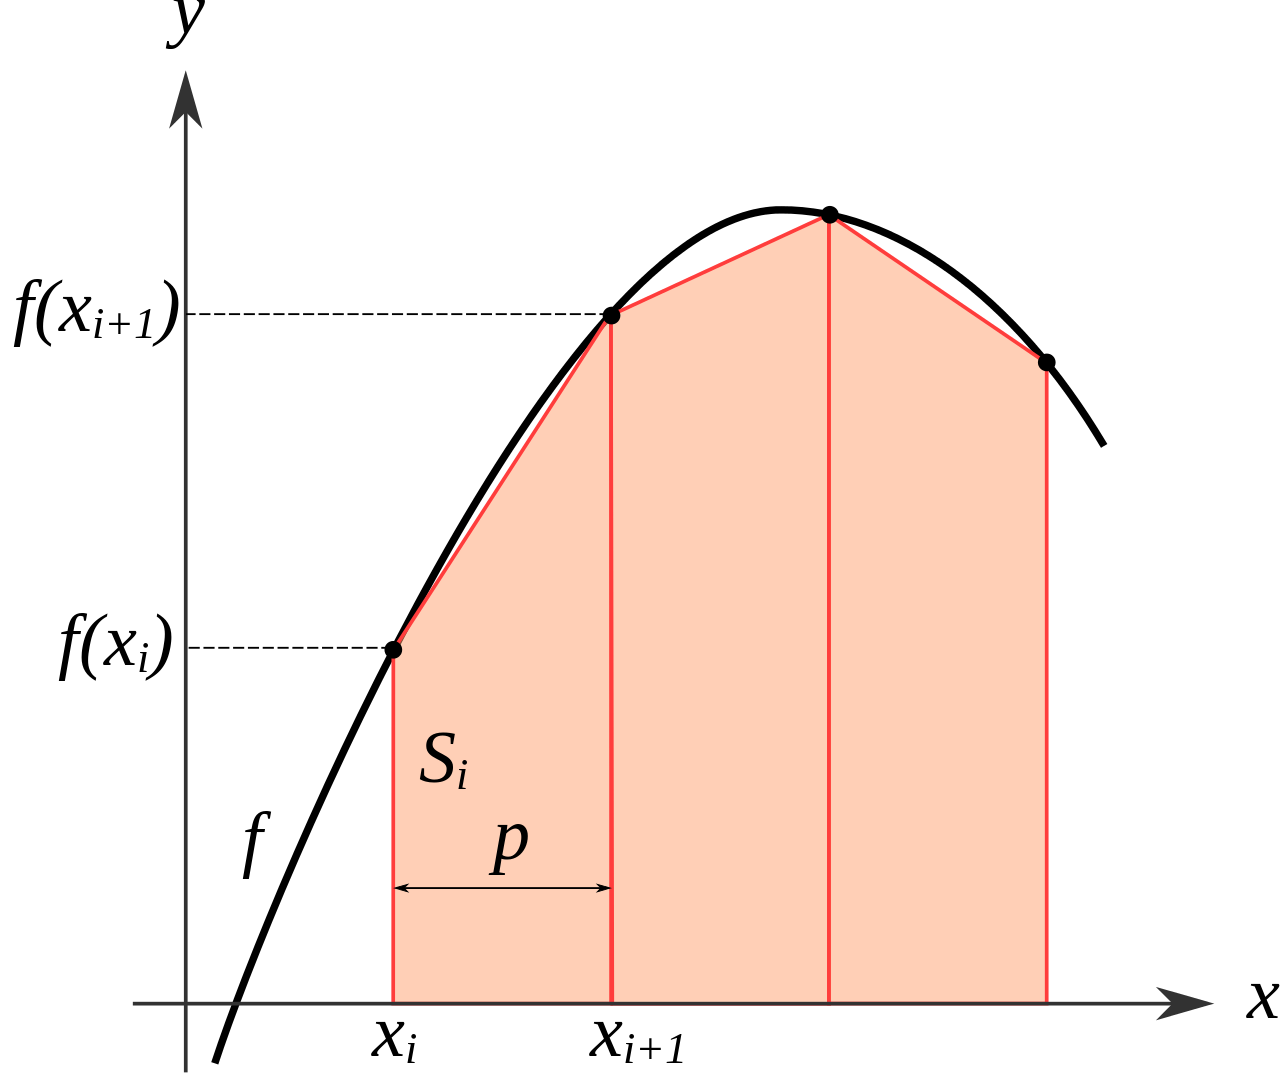
\includegraphics[width=7cm]{images/trapezoidal}
  \caption{Chained trapezoidal rule. Източник: Wikipedia\cite{trapezoidal}}
  \label{fig:trapezoidal}
  \end{centering}
\end{figure}
  

\begin{mdframed}[hidealllines=true,backgroundcolor=gray!20]
  Методът на трапеците\cite{trapezoidal} (Trapezoidal rule) е числен метод за приблежено изчисление на стойността на определения интеграл $\int_{a}^{b} f(x) dx$ на функцията $f(x)$ в интервала $[a,b]$. Същността на метода е разбиване на интервала $[a,b]$ на определен брой подинтервали $[x_i,x_{i+1}]$. За всеки подинтервал се построява правоъгълен трапец с основа $x_i x_{i+1}$ и бедра, свързващи основата с графиката на функцията в точките $f(x_i)$ и $f(x_{i+1})$ (вж. фиг. \ref{fig:trapezoidal}). Лицата на така построените трапеци се сумират, което дава приблезижение на стойността на определения интеграл. Можете да прочетете повече за метода например \href{https://en.wikipedia.org/wiki/Trapezoidal_rule}{тук}\cite{trapezoidal}.
\end{mdframed}  

\begin{enumerate}[resume]

  \item Да се дефинира функция \code{integrate(f,N)}, където $f$ е функция от тип $f:double \rightarrow double$, а $N$ е цяло положително число. \code{integrate} да конструира и връща функция $i(a,b)$ от тип $i:double \times double \rightarrow double$, изчисляваща приближено стойността на определния интеграл $\int_{a}^{b} f(x) dx$ (приемайки, че такъв съществува) по метода на трапеците, по-специално Chained trapezoidal rule\cite{trapezoidal} с $N$ на брой подинтервала.
\end{enumerate}

\pagebreak

\clearpage\section{\label{sect:llists}Линейни едносвързани списъци}

\begin{mdframed}[hidealllines=true,backgroundcolor=gray!20]
Следващите задачи са върху примерния шаблон \code{LList}, разработен на лекции. Шаблонът реализира прост контейнер чрез линеен едносвързан списък:
\begin{verbatim}
template <typename T>
struct box
{
  box(const T, box<T>*);
  box();
  T data;
  box<T>* next;
};
template <typename T>
class LList
{
public:
  LList ();
  LList (const LList<T>&);
  LList<T>& operator = (const LList<T>&);
  void push (const T&);
  void pop ();
  void insertAt (size_t, const T&);
  void deleteAt (size_t);
  void print () const;
  ~LList ();
private:
  box<T> *first;
};

\end{verbatim}
Следните задачи да се решат като упражнение за директно боравене с указателите и двойните кутии, вместо да се свеждат до използването на вече готови методи от реализацията на класа. Т.е. решенията на задачите да не ползват други методи, освен ако не са помощни функции, специално написани за тях.
\end{mdframed}

\begin{enumerate}

  \item Да се реализира метод \code{int LList<T>::count(int x)}, който преброява колко пъти елементът \code{x} се среща в списъка.

  \item Да се реализира конструктор с два аргумента $x$ и $y$ от тип $int$. Конструкторът създава списък с елементи $x, x+1, ..., y$, при положение, че $x \leq y$.

  \item Да се реализира метод \code{LList<T>::push\_back} за добавяне на елемент от тип \code{T} към \textit{края} на списъка.

  \item Да се реализира метод оператор \code{LList<T>::operator +=} за добавяне на елемент от тип \code{T} към \textit{края} на списъка.

  \item Да се реализира метод \code{LList<T>::get\_ith(int n)} за намиране на \code{n}-тия поред елемент на списъка.

  \item Да се реализира метод \code{LList<T>::push\_back} за добавяне на елемент от тип \code{T} към \textit{края} на списъка.

  \item Да се реализира метод \code{LList::removeAll (x)}, който изтрива всички срещания на елемента \code{x} от списъка.

  \item Да се реализира метод \code{$l_1$.append($l_2$)}, която добавя към края на списъка $l_1$ всички елементи на списъка $l_2$.

  \item Да се реализира метод \code{LList<T>::concat}, който съединява два списъка в нов, трети списък. Т.е. \code{$l_1$.concat($l_2$)} създава и връща нов списък от елементите на \code{$l_1$}, следвани от елементите на \code{$l_2$}.

  \item Да се дефинират оператори \code{LList<T>::operator+=} и \code{LList<T>::operator+}, съответни на методите \code{append} и \code{concat}.

  \item Да се дефинира оператор за индексиране, позволяващ четене и писане на елемент на даден индекс в списъка.

  \item Да се дефинира метод \code{LList::reverse}, който обръща реда на елементите на списъка. Например, списъкът с елементи $1,2,3$ ще се преобразува до списъка с елементи $3,2,1$.

  \item Да се дефинира функция \code{map} за списъци във функционален и деструктивен вариант.

  \item Да се дефинира функция \code{reduce} за списъци.

  \item За шаблона на клас  LList да се разработят контруктор за копиране, оператор за присвояване и деструктор. 


\end{enumerate}

\pagebreak

\clearpage\section{Клас символен низ}

\begin{mdframed}[hidealllines=true,backgroundcolor=gray!20]
Следващите задачи са върху примерния клас, реализиращ символен низ, разработен на лекции. Шаблонът реализира символен низ в динамичната памет:
\begin{verbatim}
class String
{
public:
  String ();
  String (const String<T>&);
  String (const char*);
  String& operator = (const String&);
  ~String();

  char operator [] (size_t) const;
  bool operator != (const String&) const;

  friend std::ostream &operator<<(std::ostream &, const String &);
  ~String ();
private:
  char *str;
};

\end{verbatim}
\end{mdframed}

\begin{enumerate}
  \item Да се реализира метод \code{substring (startIndex, endIndex)} на клас \code{String}, намиращ подниз с дадено начало и край.
  \item Да се реализира метод \code{substring (s)} на клас \code{String}, който намира индекса на първото срещане на подниза \code{s} в дадения низ, или \code{-1}, ако \code{s} не е подниз на дадения низ.
  \item Да се реализира метод \code{split(char separator)} на клас \code{String}. Методът да връща \code{std::vector} от символни низове (обекти от клас \code{String}), които се получават като се раздели на части дадения низ според дадения разделител. Например, низът ``\emph{Hello wold, have a nice day!}'' с разделител символа ',' ще генерира масива \{``Hello world'', `` have a nice day!''\}.
  \item Да се добавят оператори \code{+=} към класа \code{String}, позволяващи добавяне към края на низа на: символ (\code{char}), цяло число (\code{int}), булева стойност (\code{bool}).
  \item Да се добави оператор \code{=} към класа \code{String}, позволяващ на низ да се присвои произволен вектор с елементи от произволен тип \code{T}. Резултатният низ $s$ от присвояването $s=v$ да има формата ``$\{v_1,..,v_k\}$'', където $v_1,..v_k$ са представянията на елементите на $v$ като низове. Приемаме, че типа \code{T} е някой от типовете, поддържани от оператора \code{+=} на клас \code{String}.
  \item (*)Да се реализира оператор за вход от поток. \emph{Внимание: Да се съобрази, че броят на въведените символи от оператора  \code{>{}>} за \code{char[]} не е предварително известен!}

\end{enumerate}


\clearpage\section {Наследяване и полиморфизъм}

\subsection {Наследяване, виртуални методи и абстрактни класове}

\begin{enumerate}


    \item \label{zad:gamechess}Шахматни фигури.

    \begin{enumerate}[label=\alph*)]
      \item Да се дефинира структура \code{ChessPosition}, описваща коректна позиция на фигура върху шахматна дъска (‘A’-‘H’,1-8). Да се дефинира абстрактен клас \code{ChessPiece}, описващ шахматна фигура със следните операции:

      \begin{itemize}
      \item \code{ChessPosition getPosition ()}: Дава позицията на фигурата на дъската
      \item \code{[подходящ тип] allowedMoves ()}: Дава списък с всички възможни позиции, до които дадена фигура може да достигне с един ход
      \item \code{bool wins (ChessPosition)}: Проверява дали фигурата ``владее'' дадена позиция, т.е. дали позицията е в списъка с възможни ходове на фигурата
      \end{itemize}

      \item Да се дефинират класовете \code{Rook} и \code{Knight}, наследници на \code{ChessPiece}, описващи съответно шахматните фигури топ и кон.

      \item ``Стабилна конфигурация'' наричаме такава подредба на фигурите по дъската, при която никоя фигура да не е върху позволен ход на друга фигура (т.е. никои две фигури не се ``бият''). Да се дефинира функция \code{allMoves ([подходящ тип] pieces[, …])}, която по списъка \code{pieces}, съдържащ произволен брой разнородни шахматни фигури, отпечатва на конзолата всеки възможен ход на фигура от \code{pieces} такъв, че след изпълнението му списъка с фигури представлява стабилна конфигурация. Информацията за ходовете да съдържа типа на фигурата, старата позиция и новата позиция, например:

      \code{Queen A1 -> B2}

      \code{Knight B3 -> A5}

      \begin{flushleft}
      \relscale{0.85}
      Забележка: Реализирайте всички конструктори и други операции, които смятате, че са необходими на съответните класове.\\

      Забележка: Под ``списък'' се има предвид обект от класовете за линеен едносвързан списък или динамичен масив, разработени на лекции, или който е да е друг тип, който познавате и който представлява контейнер за обекти.

      \end{flushleft}

    \end{enumerate}


    \item \label{zad:boardgame}Походова игра.

    Нека GameBoard е дадена квадратна матрица \code{NxN} от цели числа, всеки елемент на която има стойност 0, 1 или 2. Елементите на матрицата със стойност 0 наричаме ``земя'', тези със стойност 1 наричаме ``огън'', а тези със стойност 2 - ``вода''. \code{GameBoard} ще наричаме ``игрова дъска''. Под ``съседна позиция'' на позицията $(i,j)$ ще разбираме тези елементи на матрицата $(i’,j’)$, такива че $|i-i’| \leq 1$ и $|j-j’| \leq 1$.

    В условието по-долу \code{N} и \code{GameBoard} да се приемат за предварително дефинирани глобални променливи.

    \begin{enumerate}[label=\alph*)]
      \item Да се дефинира структура \code{Position}, описваща позиция на игровата дъска, задаваща реда и колоната на нейн елемент. Да се дефинира абстрактен клас \code{GamePlayer}, който описва играч на игровата дъска със следните операции:

      \begin{itemize}
        \item \code{Position getPosition ()}: Дава позицията на играча на дъската
        \item \code{[подходящ тип] allowedMoves ()}: Дава списък с всички възможни позиции, до които даден играч може да достигне с един ход
        \item \code{bool wins (Position)}: Проверява дали играча ``владее'' дадена позиция, т.е. дали позицията е в списъка с възможни ходове на играча

      \end{itemize}

      \item Да се дефинира клас \code{Knight}, наследник на \code{GamePlayer}, описващ ``сухопътен рицар''. Позволените ходове на сухопътния рицар се задават със следното правило: Рицарят може да се премести в позициите, които са съседни на текущата му и които:
      \begin{itemize}
        \item са земя
        \item нямат огън в съседство
      \end{itemize}

      \item Да се дефинира клас \code{SeaMonster}, наследник на \code{GamePlayer}, описващ ``морско чудовище''. Позволените ходове на морското чудовище се задават със следното правило: Морското чудовище може да се премести във всички позиции, които са достижими от неговата при придвижване по хоризонтала или вертикала, което преминава само през вода. Например, ако вдясно от играча има три поредни позиции с вода, следвани от една позиция земя, то и трите водни позиции са достижими, но земната и всички вдясно от нея - не.
      
      \item Всяко морско чудовище да има ``сила'': цяло число $k$, което показва колко е максималния брой позиции по вертикала и хоризонтала, които чидовището може да преплува на един ход. Силата да се задава при конструиране на чудовища. 

      \item ``Стабилна конфигурация'' наричаме такава подредба на играчите по дъската, при която никой играч да не е върху позволен ход на друг играч (т.е. никои два играча не се ``бият''). Да се дефинира функция \code{allMoves ([подходящ тип] players[, …])}, която по списъка \code{players}, съдържащ произволен брой разнородни играчи, отпечатва на конзолата всеки възможен ход на играч от \code{players} такъв, че след изпълнението му списъка с играчи представлява стабилна конфигурация. Информацията за ходовете да съдържа типа на играча, старата позиция и новата позиция, например:

      \code{Knight (0,0) -> (1,1)}

      \code{SeaMonster (2,2) -> (5,2)}

      \begin{flushleft}
      \relscale{0.85}
      Забележка: Реализирайте всички конструктори и други операции, които смятате, че са необходими на съответните класове.\\

      Забележка: Под ``списък'' се има предвид обект от класовете за линеен едносвързан списък или динамичен масив, разработени на лекции, или който е да е друг тип, който познавате и който представлява контейнер за обекти.

      \end{flushleft}

    \end{enumerate}

    \item Задача 2.4.25\cite{sbornik2} В софтуерна фирма има два вида служители – програмисти и мениджъри. Отдел ``личен състав'' поддържа следната информация за всеки от програмистите:
    \begin{itemize}
      \item име;
      \item стаж (в месеци);
      \item дали знае C++;
      \item дали знае C\#
    \end{itemize}
    и следната информация за всеки от мениджърите:
    \begin{itemize}
      \item име;
      \item стаж (в месеци);
      \item колко човека управлява.
    \end{itemize}

    Да се напише програма, която позволява на отдел ``личен състав'' да поддържа списък с всички програмисти и мениджъри във фирмата. Програмата да може да извършва следните операции:
    \begin{itemize}
      \item постъпване на нов служител;
      \item напускане на служител;
      \item извеждане на списък с данни за всички служители.
    \end{itemize}

    Да се въведат примерни данни за служители  в софтуерна фирма и над тях да се изпълнят следните операции:

    \begin{itemize}
      \item изтриване на всички служители, които имат стаж по-малко от 3 месеца;
      \item записване на данните в текстов файл;
      \item прочитане на данните от текстов файл;
    \end{itemize}

\end{enumerate}

\pagebreak

\subsection{Сериализация и десериализация на контейнери. Шаблон ``Фабрика''}

\begin{enumerate}[resume]

	\item Да се сериализира и десериализира масив от масиви от числа:

	 \code{vector<vector<int> >}

	Да дефинират необходимите за целта оператори. Да се тества програмата!

	\item Да се сериализира и десериализира масив от масиви от символни низове (\texttt{char*}):

	 \code{vector<vector<char*> >}

	Да дефинират необходимите за целта оператори. Да се тества програмата!

  \item \label{zad:gamechess2}Да се разработи клас \code{ChessGame}, описващ шахматна игра с ножество от фигури по дефиницията на задача \ref{zad:gamechess} и имената на двамата играчи. Функциите за игра от задачата да се преобразуват до методи на\code{ChessGame}. Да се сериазалират и десериализират шахматни игри.

  \item \label{zad:boardgame2}Да се разработи клас \code{BoardGame}, описващ походова игра с ножество от фигури по дефиницията на задача \ref{zad:boardgame} и имената на двамата играчи. Функциите за игра от задачата да се преобразуват до методи на\code{BoardGame}. Да се сериазалират и десериализират походови игри.

	\item \label{zad:network}Да се реализира абстрактен клас \code{NetworkDevice}, който дефинира следните (абстрактни, чисто виртуални) операции:

	\begin{itemize}
		\item \code{bool attachTo(NetworkDevice* device)}: свързва устройството с друго устройство \code{device}.

		Реализациите на метода в наследниците на \code{NetworkDevice} ще връщат \code{true}, ако свързването е възможно и \code{false}, ако свързването не е възможно.  Правилата, по които се определя дали може или не може да се свърже устройството, зависят от конкретния наследник на \code{NetwrokDevice}.

		При дефиниране на метода в наследените класове осигурете, че създадената връзка е двупосочна. Т.е. счита се, че ако устройството \code{A} е свързано с устройството \code{B}, то и устройството \code{B} е свързано с устройството \code{A}. Не допускайте дадено устройство да може да се свърже повече от веднъж с едно и също устройство или пък да се свърже със себе си.

		\item \code{[попълнете правилния тип] getAttachedDevice(int i)}. Връща (\textit{Упътване: указател към}) i-тото поред устройство, към което даденото устройство е свързано и \code{nullptr}, ако индексът i не е валиден.

	\end{itemize}

	Класът \code{NetworkDevice} също да съдържа и уникален идентификатор от тип \code{int} за всяко устройство. Идентификаторът може да се задава чрез конструкторите на наследниците.

	Да се реализират производните класове \code{EndDevice} и \code{Switch}.

	\begin{itemize}
		\item За \code{EndDevice} е характерно, че устройството може да е свързано най-много с още едно устройство. Т.е. във всеки момент от времето \code{EndDevice} или не е свързан с нищо, или е свързан с точно едно устройство. Веднъж свързано, \code{EndDevice} не може да бъде свързано отново с друго устройство.

		\item За Switch е характерно, че устройството може да е свързано с максимум 8 други устройства. При достигане на броя на свързаните устройства до 8, устройството \code{Swith} не може да бъде свързвано с повече устройства.

	\end{itemize}

	Промяна на вече създадена връзка не е възможна и при двата вида устройства.

	За така дефинираните класове да се решат следните задачи:


	\begin{enumerate}[label=\alph*)]
		\item Да се реализира функция \code{void printConnections(NetworkDevice* devices[],int n)}, която отпечатва на екрана информация за връзките на всяко устройство в масив от устройства. \textit{Упътване: добавете нова виртуална функция printConncection в базовия клас. Връзките можете да печатате във формата \code{<идентификатор 1> --- <идентификатор 2>}}.

		\item Да се създаде примерна програма, в която се инициализират няколко устройства, добавят се в масив, създават се връзки между тях и се използва функцията \code{printConnections} за отпечатване на връзките.

		\item Да се реализира функция \code{bool connected([попълнете правилния тип] d1, [попълнете правилния тип] d2)}, която проверява дали има връзка (пряка или косвена) между устройствата d1 и d2. За улеснение приемете, че няма циклични връзки между устройствата. \textit{Упътване: използвайте рекурсивна функция по подобие на функциите за търсене на път.}

		\item \textit{Допълнителна задача:}Решете горната задача и при случая на възможни циклични връзки.

		\item \textit{Допълнителна задача:}Напишете функция, която по масив от устройства търси дали има циклична връзка между някои две от тях.

		\item \textit{Допълнителна задача с повишена трудност:} Сериализирайте и десериализирайте масив от свързани устройства.
	\end{enumerate}




\end{enumerate}


\pagebreak

\subsection {Виртуални конструктори и деструктори}

\begin{enumerate}[resume]
  \item За класа \code{ChessGame} от задача \ref{zad:gamechess2} да се разработят подходящи конструктори, деструктори и оператори за присвояване.
  \item За класа \code{BoardGame} от задача \ref{zad:boardgame2} да се разработят подходящи конструктори, деструктори и оператори за присвояване.
  \item Да се реализира копиране и изтриване на мрежови устройства (клас \code{NetworkDevice}) от зад \ref{zad:network}. Приемаме, че в мрежата няма цикли.
\end{enumerate}


\pagebreak

\subsection {Наследяване и агрегация. Йерархични дървета от обекти, съдържащи други обекти. Шаблон за дизайн ``Посетител.''}

\begin{mdframed}[hidealllines=true,backgroundcolor=gray!20]
  Проблемите около агрегацията на обекти от същата йерархия и получаващите се йерархични дървета от обекти, съдържащи други обекти, са демонстрирани чрез йерархия от геометрични фигури, наследници на абстрактен базов клас \code{Shape}.
  \begin{verbatim}
    class Shape
    {
    public:
        Shape ();
        Shape (int x,int y,const char *title);
        Shape (const Shape&);
        virtual Shape* clone () = 0;    
        void set_x (int);
        void set_y (int);
        void set_text (const char*);
        void operator = (const Shape& s);
        int get_x();
        int get_y();
        char* get_text();
        virtual ~Shape();
      protected:
        int x;
        int y;
        char *text;
    };
    \end{verbatim}
    
    Към йерархията е добавен клас \code{Group}, който освен че е наследник на \code{Shape}, съдържа и контейнер от наследници на \code{Shape}:

    \begin{verbatim}
      class Group: public Shape
      {
        public:
          //...
          void addShape (Shape*);
          size_t get_nChildren () const;
          Shape* getChild (size_t i) const;
          //...
          private:
          std::vector<Shape*> children;
      };
    \end{verbatim}

    За изобразяване на фигурите и сериализацията им във файл се ползва шаблонът посетител (Visitor Pattern). Всеки конкретен посетител е наследник на клас:
    \begin{verbatim}
      class Visitor
      {
      public:
          virtual void visitReactangle (Rect*) = 0;
          virtual void visitCircle (Circle*) = 0;
          virtual void visitGroup (Group*) = 0;
      };  
    \end{verbatim}

    Йерархията от фигури реализира виртуалния метод 
    
    \code{void accept (Visitor*)}, 
    
    като всяка конкретна фигура изпълнява съответния на нея метод на посетителя. По този начин се реализира т.нар. ``double dispatch''. Т.е. в следната ситуация:

    \code {figure->accept(visitor)},
    
    кой точно метод ще се изпълни се определя динамично не само според типа на обекта, сочен от \code{figure}, но и според типа на конкретния посетител, сочен от \code{visitor}. Това е изобразено на фигура \ref{fig:visitor}.
  \end{mdframed}

  \begin{figure}
    \relscale{0.5}
    \begin{tikzpicture}[auto, node distance=1.2cm,>=latex]
  
      \node  [] (title1){Rectangle};
      \node  [block,align=left,below of=title1,node distance = 0.6cm,draw] (proc1) 
        {virtual accept(Visitor*):\\visitor->process\_Rectangle(this)};
      \node[fit=(title1)(proc1), draw] (rect) {};
    
      \node  [below of = proc1] (title2){Cicrcle};
      \node  [block,align=left,below of=title2,draw,node distance = 0.6cm] (proc2) 
        {virtual accept(Visitor*):\\visitor->process\_Circle(this)};
      \node  [fit=(title2)(proc2), draw] (circ) {};
  
      \node  [below of = proc2] (title3){Group};
      \node  [block,align=left,below of=title3,draw,node distance = 0.6cm] (proc3) 
      {virtual accept(Visitor*):\\visitor->process\_Group(this)};
      \node  [fit=(title3)(proc3), draw] (group) {};
  
  
      \node  [right of = title1, node distance = 5cm] (title5){Painter};
      \node  [below of=title5,draw,node distance = 0.6cm] (proc7) {process\_Rectangle(Rectangle*)};
      \node  [below of=proc7,draw,node distance = 0.6cm] (proc8) {process\_Circle(Circle*)};
      \node  [below of=proc8,draw,node distance = 0.6cm] (proc9) {process\_Group(Group*)};
      \node  [fit=(title5)(proc7)(proc8)(proc9), draw, dashed] (paint1) {};
  
  
      \node  [below of = paint1, node distance = 2cm] (title4){Serializer};
      \node  [below of=title4,draw,node distance = 0.6cm] (proc4) {process\_Rectangle(Rectangle*)};
      \node  [below of=proc4,draw,node distance = 0.6cm] (proc5) {process\_Circle(Circle*)};
      \node  [below of=proc5,draw,node distance = 0.6cm] (proc6) {process\_Group(Group*)};
      \node  [fit=(title4)(proc4)(proc5)(proc6), draw] (ser1) {};
  
      \draw[->]  (proc1)-- (proc4);   
      \draw[->]  (proc2)-- (proc5);   
      \draw[->]  (proc3)-- (proc6);   
  
      \draw[->,dashed]  (proc1)-- (proc7);   
      \draw[->,dashed]  (proc2)-- (proc8);   
      \draw[->,dashed]  (proc3)-- (proc9);   
  
  
      %\draw[->]  (proc6.east) -| node[right of = proc6, distance=5cm]{a} (proc4.east);   
      %\draw[->] (proc6.east) -| ([xshift=1.5cm,yshift=0cm]proc5.east) |- (proc4.east);    
      %\draw[->] (proc6.east) -| ([xshift=1.5cm,yshift=0cm]proc5.east) |- (proc5.east);    
      %\draw[->]  (proc6)-- (proc5);   
  
      \node  [block,align=left,left of=proc2,draw, node distance = 4cm] (call) 
      {figure->accept(serializer)};
  
      \draw[->] (proc6.south) -| ([xshift=0cm,yshift=-1cm]proc6.south) -| (call.south); 
  
  
      \draw[->]  (call)-- (rect);   
      \draw[->]  (call)-- (circ);   
      \draw[->]  (call)-- (group);   
  
  
    \end{tikzpicture}
  
  \caption{Double Dispatch при йерархии от фигури и посетители}
  \label{fig:visitor}
  \end{figure}  


\begin{enumerate}[resume]
  \item Да се реализира десериализация на фигури чрез шаблона ``Фабрика''.
  \item Да се дефинира посетител \code{SurfaceCalculator}, който обхожда йерархия от фигури и изчисля сумата на лицата на всички фигури в нея. Приемеме, че лицето на група от фигури е равно на сумата на лицата на фигурите в групата.
  
\end{enumerate}

\pagebreak

\section{Обработка на изключения}
\begin{enumerate}

  \item Да се добавят подходящ изключенията за методите за добавяне и изтриване на елементи на линейния едносвързан списък от секция \ref{sect:llists}.

  \item \label{zad:boardex}При десериализацията на класа \code{BoardGame} от задача \ref{zad:boardgame2} да се хвърлят подходящи изключения, сигнализиращи за 
  
  \begin{itemize}
    \item Непознат тип играч
    \item Грешни данни за даден играч (напр. липсва сила за мосрко чудовище)
    \item Невъзможна конфигурация (напр. два играча на еднаква позиция)
    \item Други
  \end{itemize}

  Ако е подходящо, да се реазлизират наследници на \code{std::exception}. 
  
  Програмата да съобщава грешките на потребителя.

  (*)Какво трябва да са направи, за да се посочи реда от файла, на който е открита грешката?

  \item Решението на задача \ref{zad:boardex} да се разшири така, че да позволява възстановяване от грешки. При грешка при десериализацията на някой играч, да се изведе съобщение на потребителя и да се направи опит да се продължи с прочитането на останала част от дефиницията на играта.
  

\end{enumerate}

